%%%%%%%%%%%%%%%%%%%%%%%%%%%%%%%%%%
%%% MG 24/12/2019 - Paper notes %%%
%%%%%%%%%%%%%%%%%%%%%%%%%%%%%%%%%%

%%%% Preamble %%%%
\documentclass[a4paper, oneside]{article}

% wider text, smaller margins
\usepackage{a4wide}

\usepackage[T1]{fontenc}
\usepackage{kpfonts}

% for coloring
\usepackage[dvipsnames]{xcolor}

% for index list
\usepackage{makeidx}
\makeindex

% for compact item lists
\usepackage{paralist}

% for hyperrefs
\usepackage{hyperref}

% for declaring math operators
\usepackage{amsthm}

% wrap text around figures
\usepackage{wrapfig}

% nice text boxes
\usepackage{tcolorbox}
\newtcbox{\note}{on line, boxrule=0pt, boxsep=0pt, arc=0pt, outer arc=0pt, left=1pt, right=1pt, top=2pt, bottom=2pt, fontupper=\itshape}
\newtcolorbox{notebox}{boxrule=0pt}

% biblatex seetings for better referencing
\usepackage[backend=biber,
            citestyle=authoryear,
            bibstyle=numeric,
            block=space,
            backref=true,
            date=year,
            maxcitenames=2,
            mincitenames=1,
            url=false,
            doi=false,
            isbn=false,
            eprint=false]{biblatex}
\addbibresource{ib.bib}


%%% new shorthand commands

\newcommand{\nn}{\nonumber \\}%

\newcommand{\tldr}{\textbf{TLDR: }}
\newcommand{\concl}{\textbf{Concluding remarks: }}


% argmin/max opearator
\DeclareMathOperator*{\argmin}{arg\,min}%
\DeclareMathOperator*{\argmax}{arg\,max}%
\DeclareMathOperator*{\kl}{KL}%

% shortands for common math
\newcommand{\KL}[2]{\kl \left( #1 \parallel #2 \right)}
\newcommand{\pc}[2]{p \left( #1 \mid #2 \right)}
\newcommand{\abs}[1]{\lvert #1 \rvert}
\newcommand{\norm}[1]{\lVert #1 \rVert}
\newcommand{\dif}{\; \text{d} \, }

\newcommand{\mE}{\mathbb{E}}%%
\newcommand{\rE}{\mathrm{E}}%% % expectation
\newcommand{\rH}{\mathrm{H}}%% % entropy
\newcommand{\rI}{\mathrm{I}}%% % information
\newcommand{\mR}{\mathbb{R}}%%
\newcommand{\mcR}{\mathcal{R}}%%
\newcommand{\mN}{\mathbb{N}}%%

\newcommand{\mD}{\mathcal{D}}%%
\newcommand{\mL}{\mathcal{L}}%%
\newcommand{\mX}{\mathcal{X}}%%
\newcommand{\mY}{\mathcal{Y}}%%
\newcommand{\mZ}{\mathcal{Z}}%%

\newcommand{\bc}{\mathbf{c}}%%
\newcommand{\bx}{\mathbf{x}}%%
\newcommand{\bz}{\mathbf{z}}%%
\newcommand{\pdx}{\mathbf{p_{\mD}(\bx)}}%%



\newcommand{\bC}{\mathbf{C}}%%
\newcommand{\bX}{\mathbf{X}}%%
\newcommand{\bZ}{\mathbf{Z}}%%

% \newcommand{\note}[1]{\emph{\textbf{Note:} #1}}
% \newcommand{\idea}[1]{\emph{\textbf{\color{red}Idea:} #1}}


\begin{document}

% supress paragraph idents
\setlength{\parindent}{0pt}
\setlength{\parskip}{1ex plus 0.5ex minus 0.2ex}

% Number equations within a section
\numberwithin{equation}{section}

{\large Magda's notes about information bottleneck in learning}

{\hfill Last update: \today}

Informal notes for my future self who is likely to forget.
I explain the papers the way I understand them, using terminology and logic natural to me.
This means I may deviate from the original paper structure, notation, etc.
At places, my interpretation my be incorrect due to lack of understanding. 
I will strive for this not to happen too often but I'm certainly not infallible. 

This is a working document, not  polished, with possible typos, editing errors, etc. 


% Print table of contents
\tableofcontents

\providecommand{\hx}{}
\renewcommand{\hx}{\hat{x}}
\providecommand{\hX}{}
\renewcommand{\hX}{\hat{X}}
\providecommand{\hmX}{}
\renewcommand{\hmX}{\hat{\mX}}


\clearpage

\section{Tishby's information bottleneck method}\label{sec:ibmethod}\index{information bottleneck}

\begin{notebox}
\textbf{Paper: } \fullcite{tishbyInformationBottleneckMethod2000}

\hfill Notes taken: 25/12/2019 \index{December 2019}
\end{notebox}


\subsection{Introduction}


In this paper they use information theory, in particular the rate-distortion\index{rate-distortion theory} theory (RDT) of lossy compression, to formulate a problem of encoding a variable (signal) so that the compressed representation contains the \emph{relevant information}\index{relevant information} about some other variable.

\note{Based on \parencite{coverElementsInformationTheory2006}:}
\begin{wrapfigure}{r}{0.3\textwidth}
\vspace{-20pt}
\begin{center}
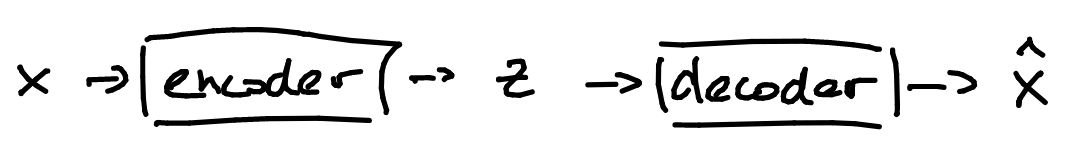
\includegraphics[width=0.3\textwidth]{autoencoder}
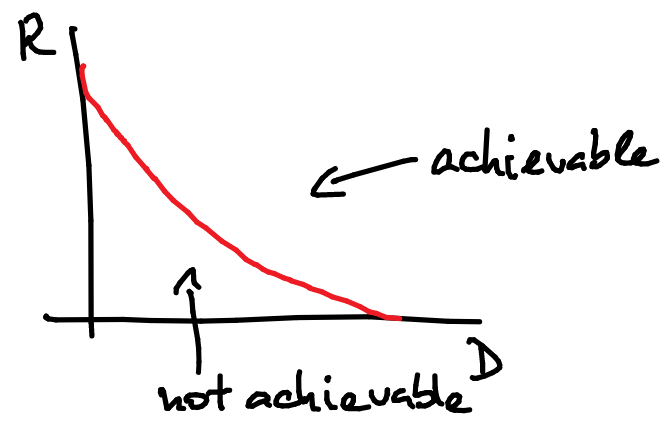
\includegraphics[width=0.25\textwidth]{RDcurve}
\end{center}
\vspace{-20pt}
\caption{\small Rate-distortion encoder and decoder and $R(D)$ curve.}
\vspace{-10pt}
\end{wrapfigure}
In the classical RDT we consider an information source\index{information source} generating sequences of i.i.d. random variables $X$ from \textbf{a known probability distribution} $X \sim p(x)$ with a finite alphabet $X \in \mX$.
We encode the source sequence $x^n \in \mX^n$ through an encoding function $f : \mX^n \to \mZ$ to an index $z \in \mZ = \{1, 2, \ldots, 2^M\}$, where $M$ is the number of bits we can use to represent the source sequence.
The decoder maps the index $z \in \mZ$ to a representation $\hx^n \in \hat{\mX}^n$ of the source sequence $x^n \in \mX^n$ through a decoding function $g : \mZ \to \hat{\mX}^n$. 
The set of possible decodings $\{g(1), g(2), \ldots, g(2^M)\}$ constitutes the \emph{codebook}\index{codebook} and $f^{-1}(z)$ are the \emph{assignment regions}\index{assignment regions}.
Replacement of $X^n$ by $\hX^n$ is commonly referred to as \emph{vector quantization}\index{vector quantization}, representation or reconstruction.

The RDT characterizes the tradeoff between the rate $R = M/n$ (average number of bits per symbol in the source sequence) and the distortion $D = \rE_{p(x)} d(X^n, f\left( g(X^n)\right)$ associated with the code.
The rate-distortion function\index{rate-distortion function} $R(D)$ determines the smallest possible rate for a given distortion $D$.
\note{I think:} If $R = \rH(X)$, this is a lossless autoencoding system where we can achieve zero distortion $D=0$.
With lower rates $R < \rH(X)$ the distortion will increase.

\note{Back to Tishby:}\\
The problem in RDT is that it does not specify which distortion functi~on $d(x, \hx)$ you shall use.\footnote{Classical examples are the squared error loss or Hamming distance.}
Once you pick it, it essentially determines which features of the signal will be considered as \emph{relevant} and encoded into $Z$. 
However, without a definition of \emph{relevance}, this is not a well posed problem. 

What they propose here is to use an additional variable $Y$ to determine what is \emph{relevant} information.
The structure of the problem is then: extract to $\hX$ the info from $X$ that is relevant for predicting $Y$. 
The choice of $Y$ will determine the \emph{relevant features} of the signal. 

\begin{notebox}
\textbf{TLDR:}
Use info theory and rate-distortion theory of encoding $X \to Z \to \hX$ to motivate encoding (compression $\approx$ feature extraction) strategy for classification problem $X \to Z \to \hX \to \hat{Y}$. Careful, $Z \in {1, \ldots, 2^M}$ is an index with $M$ determining the rate of encoding $R = M/n$ ($n$ is the length of the original sequence to be encoded). 
\end{notebox}


\subsection{Relevant quantization}

Assume signal space $\mX$ with fixed \textbf{known prob. distribution $p(x)$} and $\hmX$ its reconstruction space - quantized codebook.
\textbf{Both $\mX$ and $\hmX$ spaces are finite $\approx$ discrete or quantized (if originally continuous).}

For each $x \in \mX$ we seek a possibly \emph{stochastic} mapping to a codeword in the codebook $\hx \in \hmX$ with conditional prob. distribution $\pc{\hx}{x}$.
\begin{equation}
p(\hx) = \sum_x p(x) \pc{\hx}{x} \enspace.
\end{equation}

Average volume of elements of $\mX$ mapped to the same codeword $\hx \in \hmX$ is $2^{\rH(X \mid \hX)}$
\begin{notebox}
This comes from the entropy $\rH(X) = \rE \log_2 1/p(x)$ being the optimal length of encoding. Think of uniform $X$ with $\lvert X \rvert = c$ elements and $p(x) = 1/c$ which has entropy $\rH(X) = 1/c \sum \log_2 c = \log_2 c$.
Then volume is $\lvert X \rvert = c = 2^{\rH(X)}$
\end{notebox}

What matters for the quality of the quantization $\mX$ is a) the average number of bits per codeword $\hX \in \hmX$ and b) the expected distortion between the source and encoding $\rE_{p(x)} d(x, \hx)$. 

The average amount of information (in bits) we gain about $X$ by knowing $\hX$ (or equivalently, the reduction in the average number of bits per element in $X$ knowing $\hX$) is the mutual information
\begin{equation}
\rI(X; \hX) = \sum_{x \in \mX} \sum_{\hx \in \hmX} p(x, \hx) \log \frac{ \pc{\hx}{x} }{p(\hx)} = \rH(\hX) - \rH(\hX \mid X)  = \rH(X) - \rH(X \mid \hX) \enspace .
\end{equation}
For stochastic mappings $\rH(\hX \mid X) \neq 0$ and $\rH(\hX)$ is not what we want to minimize.

\begin{notebox}
\tldr Treat source $\mX$ and reconstruction $\hmX$ spaces as discrete. Allow for stochastic mapping (encoding-decoding) $p(\hx | x)$. Good reconstruction should have high mutual information with the source $\rI(X; \hX) = \sum_{x \in \mX} \sum_{\hx \in \hmX} p(x, \hx) \log \frac{ \pc{\hx}{x} }{p(\hx)}$.
\end{notebox}

\subsection{Relevance through distortion}

The ability to reconstruct is measured in RDT by the distortion function $\mX \times \hmX \to \mR_{+}$ with expected distortion 
\begin{equation}
D = \rE_{p(x, \hx)} d(x, \hx) = \sum_{x \in \mX} \sum_{\hx \in \hmX} d(x, \hx)
\end{equation}
which is presumed to be low for good reconstructions $\hX$ and which implicitly specifies what are the most \emph{relevant} aspects of $X$.

There is a monotonic trade-off between the rate R and the distortion D described by the rate-distortion function $R(D)$\index{rate-distortion function}.
The $R(D)$ function is defined as the minimal achievable rate (mutual information) with a given constraint $D^*$ on the expected distortion
\begin{equation}
R(D) := \min_{\pc{\hx}{x}: \rE_{p(x, \hx)} d(x, \hx) \leq D^*} \rI(X; \hX)
\end{equation}
or in the Lagrangian form as the minimization of 
\begin{equation}
\mL[ \pc{\hx}{x}] = \rI(X; \hX) + \beta \rE_{p(x, \hx)} d(x, \hx) \enspace ,
\end{equation}
where $\beta = -\frac{\dif R}{\dif D} > 0$

For each $\beta$ (that is for each distortion constraint $D^*$) the $\pc{\hx}{x}$ can be found by \emph{Blahut-Arimoto algorithm}\index{Blahut-Arimoto algorithm} which alternates between ensureing that $p(\hx) = \sum_x p(x) \pc{\hx}{x}$ and minimizing the RDT objective.
It's important to note that it only finds the optimal partitioning $\pc{\hx}{x}$ over a given representation space $\hX$.
Finding optimal space $\hX$ would need some sort of EM algorithm.

\begin{notebox}
\tldr In RDT we ere looking for $\pc{\hx}{x}$ which minimizes the mutual information $\rI(X; \hX)$ (minimizes the rate $\approx$ maximizes the compression) with a limit on the expected distortion $\rE_{p(x, \hx)} d(x, \hx) \leq D^*$. This can be formulated as the minimization of 
\begin{equation}
\mL[ \pc{\hx}{x}] = \rI(X; \hX) + \beta \rE_{p(x, \hx)} d(x, \hx) \enspace .
\end{equation}
\end{notebox}

\subsection{Relevance through other variable - information bottleneck}\index{information bottleneck}

As before, we want the quantization $\hX$ to compress $X$ as much as possible but instead of looking at distortion $d(x, \hx)$, we will look at how much information about some third variable $Y$ the quantization $\hX$ can capture $\rI(\hX, Y)$.
We assume that the original signal has positive mutual information with the variable $\rI(X; Y)$ and that the \textbf{true joint distribution $p(x, y)$ is known.}

As lossy compression cannot convey more information than the original data we have $\rI(\hX; Y) \leq \rI(X; Y)$.
The trade-off we look for now is between the rate $\rI(X; \hX)$ (compression) while preserving meaningful info about $Y$: we pass the information $X$ has about $Y$ through a \emph{bottleneck} representation $\hX$.

Similarly to before, we find the optimal $\pc{\hx}{x}$ by minimizing the functional
\begin{equation}
\mL[ \pc{\hx}{x}] = \rI(X; \hX) - \beta \rI(\hX; Y) \enspace ,
\end{equation}
where instead of minimizing the expected distortion $\rE_{p(x, \hx)} d(x, \hx)$ we maximize the mutual information $\rI(\hX; Y)$.

They then proof using the machinery of the Blahut-Arimoto algorithm that the optimal solution is 
\begin{equation}
\pc{\hx}{x} = \frac{p(\hx)}{Z(x, \beta)}
\exp \left[ -\beta \KL{\pc{y}{x}}{\pc{y}{\hx}} \right] \enspace ,
\end{equation}
where $Z(x, \beta)$ is the normalization constant (nothing to do with the encoder $\mZ$.)
This suggest the KL divergence is the \emph{correct} distortion measure in this seeting.
They further propose an algorithm which is alternating between optimizing $\pc{\hx}{x}$, and making sure $p(\hx)$ and $\pc{y}{\hx}$ are consistent with it and the known $p(x, y)$.

\begin{notebox}
\tldr Use some other variable $Y$ with $\rI(X; Y) > 0$ to guide the quality of the representation $\hX$. It should still compress (with low $\rI(X; \hX)$) but instead of $d(x, \hx)$ use $\rI(\hX; Y)$ to see how much the representation preserves from $Y$. The optimization is 
\begin{equation}
\mL[ \pc{\hx}{x}] = \rI(X; \hX) - \beta \rI(\hX; Y) \enspace ,
\end{equation}
and the solution is alternating algo similar to Arimoto-Blahut.
\end{notebox}

\begin{notebox}
\concl 
It is not clear to me what (if anything) can break if we move from the discrete case considered here to the continuous case.
But, more importantly, the assumption that we have access to the true distribution $p(x, y)$ certainly does not hold in ML.
\end{notebox}


\providecommand{\hx}{}
\renewcommand{\hx}{\hat{x}}
\providecommand{\hX}{}
\renewcommand{\hX}{\hat{X}}

\clearpage

\section{Tishby's information bottleneck principle in DL}\label{sec:ibdnn}\index{information bottleneck}

\begin{notebox}
\textbf{Paper: } \fullcite{tishbyDeepLearningInformation2015}

\hfill Notes taken: 25/12/2019 \index{December 2019}
\end{notebox}


\subsection{Introduction}

They formulate the goal of deep learning as an information theoric trade-off between compression and prediction (building on the information bottleneck method \ref{sec:ibmethod}) and give some guarantees for generalization.

\subsubsection{The DNN setting}
They consider MLPs with sigmoid neurons, high dimensional inputs $X$ and classification (multi-class) output $Y$.
The optimisation is performed by SGD through backpropagation of some loss.

\subsubsection{The information bottleneck principle}

The principle suggests to encode $X$ into $\hX$ such that it squeezes out of $X$ all information not relevant for predicting $Y$.
$\hX$ can be seen as the minimal sufficient statistic of $X$ with respect to $Y$, ot the simplest representation of $X$ that captures the mutual info $\rI(X; Y)$.
For the classification case they assume a Markov chain $Y \to X \to \hX$ with conditional independence assumption $Y \perp \hX \mid X$ described by the joint density $p(y, x, \hx) = p(y) \pc{x}{y} \pc{\hx}{x} $ and the data processing inequality (DPI)\index{data processing inequality} $I(Y; X) \geq I(Y; \hX)$.

The information bottleneck (IB) method proposes to learn the stochastic mapping $\pc{\hx}{x}$ by minimizing
\begin{equation}
\mL[ \pc{\hx}{x}] = \rI(X; \hX) - \beta \rI(\hX; Y) \enspace .
\end{equation}
They suggest to reformulate it reformulate it as the minimization
\begin{equation}\label{ibdmm:optim}
\mL[ \pc{\hx}{x}] = \rI(X; \hX) + \beta \rI(X; Y \mid \hX) \enspace ,
\end{equation}
that is minimizing the residual information about $Y$ in $X$ not captured by $\hX$.

\subsubsection{IB for DNN}

They see the DNN layers as forming a Markov chain $Y \to X \to h_1 \to \ldots \to h_n \to \hat{Y}$ in which the DPI holds $\rI(Y; X) \geq \rI(Y; h_1) \geq \ldots \geq \rI(Y; h_n) \geq \rI(Y; \hat{Y})$, where equality holds only if each layer is sufficient statistic of its input with respect to $Y$.

From learning perspective, each layer should try to minimize $\rI(h_{i-1}; h_i)$ while maximizing $\rI(Y; h_i)$.
They have got some bounds on the prediction error based on $\rI(Y; h_i)$.
Also the optimal theoretical limit of equation \eqref{ibdmm:optim} can be evaluated for each intermediate layer conditioning on the previous layers.
Each consecutive layer compresses the inputs increasing the distortion.

\subsubsection{Generalization bounds}

The IB curve obtained by minimizing \eqref{ibdmm:optim} is a property of a joint distribution $p(x, y)$ which is unknown in ML.
Assuming bouinded cardinality of the representation $K = \abs{\hX}$ (that is of the layers $h_i$) the difference between the true mutual information $\rI(X; \hX)$ resp. $\rI(\hX; Y)$ and their sample estimates increases with $K$ but not with the cardinality of $X$.
Which means the IB curve can be well estimated for compressed representations but badly estimated for complex representations.
Using these bounds, they sketch worst-case bound on the out-of-sample RD curve which actually has an optimal point with minimal distortion and corresponding rate. 
They claim that as the compression progresses we move closer in the information plane to this optimal point.
 
\begin{notebox}
\tldr Transfer the information bottleneck method to DNN classification learning.
For compressed representation $\hX$ of the signal $X$ and the target $Y$ the optimization problem is
\begin{equation}
\mL[ \pc{\hx}{x}] = \rI(X; \hX) + \beta \rI(X; Y \mid \hX) \enspace .
\end{equation}
In the DNN case each hidden layer $h_i$ is seen as the compressed representation $\hX$ so that we have the following DPI  $\rI(Y; X) \geq \rI(Y; h_1) \geq \ldots \geq \rI(Y; h_n) \geq \rI(Y; \hat{Y})$.
They also have some generalization bounds claiming that what matters is the cardinality of the representations $K = \abs{\hX}$ but not of $\abs{X}$. 
\end{notebox}

\begin{notebox}
\concl Rather straightforward extension of IB method to DNNs. I`m not sure how reasonable is the generalization analysis (haven't read the other paper they wrote and cite) but it seems to somehow rely on the discrete nature of the source and encoding spaces which is gnerally not true in DL.
\end{notebox}


\clearpage

\section{Tishby's information theory of DL}\label{sec:infoDL:_Tisby}\index{information bottleneck}

\begin{notebox}
\textbf{Video: } \fullcite{tishbyInformationTheoryDeep2017}

\hfill Notes taken: 26/12/2019 \index{December 2019}
\end{notebox}

Bringing information theory into classification problems solved by DL.

Transferring information bottleneck method and data processing inequality (DPI) into the learning. The DPI basically says that for any three random variables in a Markov chain Y->X->H we have $\rI(Y, X) \geq \rI(Y, H)$. Thinking about hidden layers H as useful compression, we should try to compress H to reduce as much as possible $\rI(X,H)$ while keeping $\rI(H,Y)$ $\approx$ information bottleneck method.

He is very keen to replace the standard PAC learning theory by his IB based theory so he is well aware of the problem of generalization. But I don't find in his talk any really convincing arguments. He simplifies so much that in the end it seem he is missing the point.

He has plenty of stories about how what we see in training is first a drift of the layers to remember the data followed by a stage of compression. It all seems to me like a somewhat far-fetched try to push the coding theory onto the learning. But for it to work you would need to shift the DL training from \note{continuous to discrete} problem and instead of the nets being \note{deterministic}, have them as \note{stochastic}.

It seems to me that plenty of what he shows is rather the \note{result of his evaluation procedure}, e.g. the binning which suggests loss of information while in the continuous case no info is lost and some sort of clustering which again never really happens and rather the Bayes decision rule is applied over the continuous outputs.

\note{Other questions:} As he says, each of the layers is just a deterministic transformation of the previous layer which is moreover in the case of simple nonlinearities such as sigmoid or tanh invertible. He also says that mutual information is invariant under invertible transformations $\rI(X, Y) = \rI(f(X), g(Y))$. If both of these are true, how could any information be lost?

He also admits that the learning rule cannot be completely deterministic because otherwise his theory breaks and that they kind of get away from it by the binning. But this is not what really happens. What in his talk is real effect and what just evaluation artifact?

He argues by typicality that the network actually learns some clusters. I can see the network learns clusters but the typicality arguments seem far-fetched.

The usual coding theory is based on knowing the true $p(x,y)$ distribution but we only observe samples of it. He admits this is a problem but almost trivializes this too much.

He has a graph showing how during the training gradients first have high mean and small std (across the batches within epoch) and some point shift to low means and high gradients. I find this perfectly natural. The network first needs to learn so all gradients are high and not too different as all the updates from all the batches push the weights to something reasonable. After this happens, the gradients become smaller in mean (reaching a plateau so don't need so big changes) but each batch suggests a move in different direction. In my head this does not necessarily have to do anything with compression, just the way the optimization happens.



\clearpage

\section{Saxe (Harvard): IB in DL - critique of Tishby's findings}\label{sec:ibDL}\index{information bottleneck}

\begin{notebox}
\textbf{Paper: } \fullcite{saxeInformationBottleneckTheory2018}

\hfill Notes taken: 26/12/2019 \index{December 2019}
\end{notebox}

They question the conclusions of \parencite{tishbyInformationTheoryDeep2017} (see section \ref{sec:infoDL:_Tisby}) who claims that a) DL training consists of two phases - fitting followed by compression, b) it is due to the compression phase that DN don't overfit, c) the compression appears due to diffusion-like effect of SGD. Here they show that none of these is generally true (mainly empirically with some theory behind but not too elaborate). The compression that Tishby observed is more due to nonlinearity they used (tanh) which has a double-sided saturation effect (unlike ReLu which is unbounded on one side). They also show that you can have good generalization without compression and that compression does not arise from stochasticity of SGD but can arise in batch as well.

There is a discussion related to the evaluation of the mutual information which usually calculates the info and entropy metrics as if the variables were discrete (through binning) but since they are not, this is just an arbitrary bias introduced to the evaluation.

Also, for deterministic functions $f$ the mutual information $\rI(X, h=f(X))$ is infinity, it is in general impossible to analyse mutual info of the deterministic NN layers without introducing some error.

\begin{notebox}
\concl The paper caused quite a lot of controversy around the IB method by criticising initial Tishby's findings. Though they often present similarly flawed results (little theory, basic experiments) they pose the right questions and open room for discussion.
\end{notebox}



\clearpage

\section{Goldfeld (MIT): Estimating Info Flow in DNNs}\label{sec:estimInfoFlowDL}\index{information flow}

\begin{notebox}
\textbf{Paper: } \fullcite{goldfeldEstimatingInformationFlow2019}

\hfill Notes taken: 26/12/2019 \index{December 2019}
\end{notebox}

Coming back to recent papers of \cite{shwartz-zivOpeningBlackBox2017,saxeInformationBottleneckTheory2018} they recognize that using mutual information $\rI(.;.)$ for measuring the effect of learning does not make sense in non-stochastic setting because it is either constant (in the discrete setting) or infinite (in the continuous).
Furthermore, the compression effect empirically observed in the previous papers is likely an artefact of the estimation procedure of $\rI(.;.)$ relying on binning the neuron output space.

To address this they propose a stochastic DNN framework where each neuron output is contaminated by Gaussian noise.
This makes $\rI(.;.)$ express something reasonable \emph{(though to me it seems just making the problem even more contrived because what we will be measuring is somehow the resiliency to the imputed noise)}.
$\rI(.;.)$ still has no exact analytical expression due to the complex transformations of the variables (and the distributions) in the DNN.

They propose an estimator of $\rI(.;.)$ (based on their previous work) which uses the empirical estimates of the differential entropies of the Gaussian noisy signals (Gaussian noisy channel in the info theory jargon)\index{noisy channel}.
These rely on the fact that the data sample is i.i.d. and therefore entropy estimates should converge to the true differential entropies with enough samples. They still need some Monte Carlo integration to really evaluate the entropies but they don't elaborate. Obviously, the number of samples is critical and they do admit it but provide results for manageable sample sizes claiming they should be good enough.

Finally, they empirically explore the behaviour of the mutual information $\rI(X; T_k)$ and the entropy $\rH\left( binned(T_k)\right)$, where $T_k$ is the layer output after adding the noise.
They conclude that what is actually happening during the training across the layers is better and better clustering to finally correspond to the output categories.
The compression previously observed was actually this clustering which is naturally captured in the bin-based entropy but not in the true mutual information, and certainly not in the deterministic case when measuring mutual info makes no sense.
Furthermore, compression measured through mutual information does not seem to causally relate to generalization.
The clustering effect of the layers (its geometry) is worth further study.

\begin{notebox}
\tldr Mutual information is useless for tracing learning through layers of deterministic nets (it's constant for discrete and infinite for continuous).
What has been previously observed as compression is artefact of estimating differential entropy via binning.
The binning estimates clustering within the transformed space and it is the clustering effect which is important for accuracy and generalization (not the compression measured by mutual information). Whatever the previous papers were saying about compression holds if you \textbf{replace compression with clustering}.
\end{notebox}

\begin{notebox}
\concl To me the clustering effect of the neurons and layers seems so obvious that I find it difficult to believe no one discussed it before.
However, if you think about clustering it is a form of compression so one needs to be careful about the terminology.
Perhaps rather than clustering, what is happening is some sort of concentration, mode creation in the distributions?
Well, this is sort of clustering as well (aka Gaussian mixture).
\end{notebox}



\providecommand{\qfz}{}
\renewcommand{\qfz}{q_\phi( \bz \mid \bx)}
\providecommand{\ptc}{}
\renewcommand{\ptc}{p_\theta( \bc \mid \bz)}
\providecommand{\ptx}{}
\renewcommand{\ptx}{p_\theta( \bx \mid \bz)}
\providecommand{\pxz}{}
\renewcommand{\pxz}{p_\xi(\bz)}

\clearpage

\section{Slava's WP linking VAEs and GANs through information bottleneck}\label{sec:ibvariational}\index{information bottleneck}\index{Slava}


\begin{notebox}
\textbf{Paper: } \fullcite{voloshynovskiyInformationBottleneckVariational2019}\index{Slava}\index{information bottleneck}

\hfill Notes taken: 26/12/2019 \index{December 2019}
\end{notebox}

\begin{notebox}
\textbf{Warning:} In this summary I deviate quite a bit from the original paper because the original structure and notation is difficult to follow.
\end{notebox}

\subsection{Introduction}

They aim at transferring the IB method from supervised learning to unsupervised learning of the VAE and GAN family and try to link all these together by formulating unified learning objectives.
This is achieved through various decomposition and reformulations of the original IB method (not really achieved for GANs, in my view.)

\begin{notebox}
\textbf{Thought:} The IB supervised method was initially motivated by the unsupervised rate-distortion coding. Isn't this a bit running in circles?
\end{notebox}

\subsection{IB for supervised models}

Standard supervised classification setup with observations $\{(\bx_i, \bc_i) \in \mR^d \times \mathcal{M}\}_{i=1}^N$ assuming true generative process $p(\bx, \bc) = p(\bc)\pc{\bx}{\bc}$.

According to Tishby's bottleneck method \parencite{tishbyInformationBottleneckMethod2000, tishbyDeepLearningInformation2015} (see sections \ref{sec:ibmethod}, \ref{sec:ibdnn}) the optimization problem is the minimization of the functional 
\begin{align}\label{ibvar:optimsuper}
\mL^{S}[\qfz] 
& := \rI_{\phi}(\bX; \bZ) - \beta \rI(\bZ; \bC) \nn
& = \rH_\phi(\bZ) - \rH_\phi(\bZ \mid \bX) - \beta \left( \rH(\bC) - \rH_\phi(\bC \mid \bZ) \right) 
 \enspace ,
\end{align}
where $\bZ$ is a representation of $\bX$ with a learned probabilistic mapping $\qfz$ and Markov chain condition $\bC \to \bX \to \bZ$ so that $(\bZ \perp \bC) \mid \bX$.

In the original Tishby's paper it was assumed that the true generative distribution $p(\bx, \bc)$ and the support sets of $\bX$ and $\bZ$ \textbf{\emph{are known}} and they are both finite (i.e. discrete random vars).
However, here they use integrals which means they assume continuous $\bX$ and $\bZ$ which corresponds better to DL (but I'm not sure what are the consequences for the mutual info which breaks for deterministic mappings).

The following relations are needed for the entropy evaluations in \ref{ibvar:optimsuper}) hold
\begin{gather}
p(\bx, \bc) = p(\bc)\pc{\bx}{\bc} \qquad \pc{\bc}{\bx} = \frac{p(\bx, \bc)}{p(\bx)} \nn
p_\phi(\bx , \bz) = p(\bx) \qfz \qquad p_\phi(\bz) = \int_\bx p(\bx) \qfz \dif \bx \qquad 
p_\phi(\bx \mid \bz) = \frac{p(\bx) \qfz}{\int_\bx p(\bx) \qfz \dif \bx} \nn
p_\phi(\bc , \bz) 
= \int_\bx \pc{\bc}{\bx} p_\phi(\bx, \bz) \dif \bx = \int_\bx \frac{p(\bx, \bc)}{p(\bx)} p(\bx) \qfz \dif \bx 
=  \int_\bx p(\bx, \bc) \qfz \dif \bx \nn
p_\phi(\bc \mid \bz) = \int_\bx \pc{\bc}{\bx} p_\phi(\bx \mid \bz) \dif \bx 
=  \int_\bx  \frac{p(\bx, \bc)}{p(\bx)} \frac{p(\bx) \qfz}{\int_\bx p(\bx) \qfz \bx} \dif \bx
= \int_\bx  \frac{p(\bx, \bc) \qfz}{\int_\bx p(\bx) \qfz \dif \bx} \dif \bx
\nonumber
\end{gather}

\begin{gather}
\rH_\phi(\bZ)  = - \int_\bz p_\phi(\bz) \log p_\phi(\bz) \dif \bz
= - \int_\bz \int_\bx p(\bx) \qfz \log \left( \int_\bx p(\bx) \qfz \dif \bx \right) \dif \bx \dif \bz
\nn
\rH_\phi(\bZ \mid \bX) = - \int_\bx \int_\bz  p(\bx) \qfz \log \qfz \dif \bz \dif \bx 
\qquad 
\rH(\bC) = - \sum_\bc p(\bc) \log p(\bc)
\nn 
\rH_\phi(\bC \mid \bZ)
 = - \int_\bz \sum_\bc p_\phi(\bz) p_\phi(\bc \mid \bz) \log p_\phi(\bc \mid \bz) \dif \bz 
 = - \int_\bz \int_\bx \sum_\bc p(\bx, \bc) \qfz \log p_\phi(\bc \mid \bz) \dif \bx \dif \bz \nn
 = - \int_\bz \int_\bx \sum_\bc p(\bx, \bc) \qfz \log \left( \int_\bx  \frac{p(\bx, \bc) \qfz}{\int_\bx p(\bx) \qfz \dif \bx} \dif \bx \right) \dif \bx \dif \bz \nonumber
\end{gather}
For the moment, we cannot evaluate any of the above entropies and learn $\qfz$ because a) the true generative distribution is unknown, b) integrations over the $\bX$ and $\bZ$ spaces.

In the next step they introduce a learnable approximation to the classification distribution $p_\phi(\bc \mid \bz) \approx \ptc$ parametrized by $\theta$ (they don't really explain why) with a cross-entropy $\rH_{\phi, \theta}(\bC \mid \bZ)$
\begin{gather}
\rH_\phi(\bC \mid \bZ) \leq \rH_{\phi, \theta}(\bC \mid \bZ)
= - \int_\bz \int_\bx \sum_\bc p(\bx, \bc) \qfz \log \ptc \dif \bx \dif \bz 
\nn
\rH_{\phi, \theta}(\bC \mid \bZ) - \rH_\phi(\bC \mid \bZ) =
\int_\bz p_\phi(\bz) \KL{p_\phi(\bc \mid \bz)}{\ptc} \dif \bz
\enspace ,
\end{gather}
where the inequality holds by standard properties of cross-entropy and the positive KL.

They replace the classification entropy with the cross-entropy in the objective function \ref{ibvar:optimsuper} to obtain an upper bound which can be minimized instead
\begin{equation}
\mL^S[\qfz] \leq \mL^{SB}[\qfz, \ptc] := \rH_\phi(\bZ) - \rH_\phi(\bZ \mid \bX) + \beta \rH_{\phi, \theta}(\bC \mid \bZ) - \beta \rH(\bC) .
\end{equation}
Note that the last term is constant (though unknown) and can be dropped from the optimization objective.
Also note that for any pair $(\qfz, \ptc)$ (including the optimal) we have
\begin{equation}
\mL^{SB}[\qfz, \ptc] = \mL^S[\qfz] + \int_\bz p_\phi(\bz) \KL{p_\phi(\bc \mid \bz)}{\ptc} \dif \bz
\end{equation}

\begin{notebox}
\tldr Start from Tishby's IB method objective for classification problem.
In addition to learning the $\phi$ parameter of the representation stochastic mapping $\qfz$, learn also the $\theta$ parameters of the variational approximation to the classification entropy $\ptc \approx p_\phi(\bc \mid \bz)$.
Instead of optimising the original objective $\mL^S[\qfz]$, minimise its upper bound 
\begin{align}
\mL^{SB}[\qfz, \ptc] & = \mL^S[\qfz] + \int_\bz p_\phi(\bz) \KL{p_\phi(\bc \mid \bz)}{\ptc} \dif \bz \nn
& = \rH_\phi(\bZ) - \rH_\phi(\bZ \mid \bX) + \beta \rH_{\phi, \theta}(\bC \mid \bZ) \nonumber \enspace ,
\end{align}
where $\rH_{\phi, \theta}(\bC \mid \bZ)
= - \int_\bz \int_\bx \sum_\bc p(\bx, \bc) \qfz \log \ptc \dif \bx \dif \bz$ is the cross-entropy for ecoding $\ptc$ via $p_\phi(\bc \mid \bz)$.
It is not clear how this problem can be optimised. 
\end{notebox}


\subsection{Information bottleneck for unsupervised problem}
The set-up changes in that we only observe samples of $\bX \sim p(\bx)$ and want to predict $\bX$ from the representation $\bZ$.

Essentially, they replace $\bC$ with $\bX$ in all the above.

The original objective is 
\begin{align}\label{ibvar:optimunsuper}
\mL^{U}[\qfz] 
& := \rI_{\phi}(\bX; \bZ) - \beta \rI(\bZ; \bX) \nn
& = \rH_\phi(\bZ) - \rH_\phi(\bZ \mid \bX) - \beta \left( \rH(\bX) - \rH_\phi(\bX \mid \bZ) \right) 
 \enspace ,
\end{align}
with the following relations
\begin{gather}
p_\phi(\bx , \bz) = p(\bx) \qfz \qquad p_\phi(\bz) = \int_\bx p(\bx) \qfz \dif \bx \qquad 
p_\phi(\bx \mid \bz) = \frac{p(\bx) \qfz}{\int_\bx p(\bx) \qfz \dif \bx} \nonumber
\end{gather}
\begin{gather}
\rH_\phi(\bZ)  = - \int_\bz p_\phi(\bz) \log p_\phi(\bz) \dif \bz
= - \int_\bz \int_\bx p(\bx) \qfz \log \left( \int_\bx p(\bx) \qfz \dif \bx \right) \dif \bx \dif \bz
\nn
\rH_\phi(\bZ \mid \bX) = - \int_\bx \int_\bz  p(\bx) \qfz \log \qfz \dif \bz \dif \bx 
\qquad 
\rH(\bX) = - \int_\bx p(\bx) \log p(\bx)
\nn 
\rH_\phi(\bX \mid \bZ)
 = - \int_\bz \int_\bx p_\phi(\bz) p_\phi(\bx \mid \bz) \log p_\phi(\bx \mid \bz) \dif \bz 
 = - \int_\bz \int_\bx p(\bx) \qfz \log p_\phi(\bx \mid \bz) \dif \bx \dif \bz \nn
 = - \int_\bz \int_\bx p(\bx) \qfz \log \left( \frac{p(\bx, \bc) \qfz}{\int_\bx p(\bx) \qfz \dif \bx} \right) \dif \bx \dif \bz \nonumber
\end{gather}

Next they introduce the learnable approximation $\ptx \approx p_\phi(\bx \mid \bz)$ parametrized by $\theta$ with the cross-entropy $\rH_{\phi, \theta}(\bX \mid \bZ)$
\begin{gather}
\rH_\phi(\bX \mid \bZ) \leq \rH_{\phi, \theta}(\bX \mid \bZ)
= - \int_\bz \int_\bx p(\bx) \qfz \log \ptx \dif \bx \dif \bz 
\nn
\rH_{\phi, \theta}(\bX \mid \bZ) - \rH_\phi(\bX \mid \bZ) =
\int_\bz p_\phi(\bz) \KL{p_\phi(\bx \mid \bz)}{\ptx} \dif \bz
\enspace .
\end{gather}

Finally, they plug this into the objective so that
\begin{equation}\label{ibvar:otimunsuperb}
\mL^U[\qfz] \leq \mL^{UB}[\qfz, \ptx] := \rH_\phi(\bZ) - \rH_\phi(\bZ \mid \bX) + \beta \rH_{\phi, \theta}(\bX \mid \bZ) - \beta \rH(\bX).
\end{equation}
The last constant (though unknown) term can again be dropped and we also have the bound relation for any pair $(\qfz, \ptx)$ (including the optimal)
\begin{equation}
\mL^{UB}[\qfz, \ptx = \mL^U[\qfz] + \int_\bz p_\phi(\bz) \KL{p_\phi(\bx \mid \bz)}{\ptx} \dif \bz
\end{equation}

\begin{notebox}
\tldr In the unsupervised setting we only have $\bX \sim p(\bx)$ but will use exactly the same machinery for predicting (reconstructing) $\bX$ from $\bZ$ as in the supervised setting simply by replacing $\bC$ with $\bX$ everywhere.
We learn the distribution $\qfz$ and the variational approximation $\ptx \approx p_\phi(\bx \mid \bz)$ by minimising
\begin{align}
\mL^{UB}[\qfz, \ptx] & = \mL^U[\qfz] + \int_\bz p_\phi(\bz) \KL{p_\phi(\bx \mid \bz)}{\ptx} \dif \bz \nn
& = \rH_\phi(\bZ) - \rH_\phi(\bZ \mid \bX) + \beta \rH_{\phi, \theta}(\bX \mid \bZ) \nonumber \enspace ,
\end{align}
with $\rH_{\phi, \theta}(\bX \mid \bZ)
= - \int_\bz \int_\bx p(\bx) \qfz \log \ptx \dif \bx \dif \bz$.
\end{notebox}

\subsubsection{Rewriting the objective}

We can rewrite the final objective \ref{ibvar:otimunsuperb} as
\begin{align}
\mL^{UB}[\qfz, \ptx] = &
- \int_\bz \int_\bx p(\bx) \qfz \log \frac{p_\phi(\bz)}{\qfz} \dif \bx \dif \bz \nn
& - \beta \int_\bz \int_\bx p(\bx) \qfz \log \ptx \dif \bx \dif \bz
\end{align}

They introduce another variational approximation $\pxz \approx p_\phi(\bz)$, this time of the marginal of $\bZ$, and bring it into the objective
\begin{gather}
\mL^{UB}[\qfz, \ptx, \pxz] = 
- \mE_{p(\bx)} \mE_{\qfz} \log \frac{p_\phi(\bz) \pxz}{\pxz \qfz}
- \beta \mE_{p(\bx)} \mE_{\qfz} \log \ptx \nn
= 
\mE_{p(\bx)} \KL{\qfz}{\pxz} - \KL{p_\phi(\bz)}{\pxz}
- \beta \mE_{p(\bx)} \mE_{\qfz} \log \ptx \nonumber
\end{gather}

Finally they introduce an estimate of the true data density $p_\varphi(\bx) \approx p(\bx)$ and simply plug into the objective a KL divergence to minimize the distance between the two (which is equivalent to maximizing the log likelihood $\mE_{p(\bx)}\log p_\varphi(\bx)$) making the objective yet another upper bound on the original (we minimize the objective)
\begin{gather}
\mL^{U}[\qfz] \leq \mL^{UB}[\qfz, \ptx] \leq \mL^{UBD}[\qfz, \ptx, \pxz, p_\varphi(\bx)] := \nn
\underbrace{\mE_{p(\bx)} \KL{\qfz}{\pxz}}_A - \underbrace{\KL{p_\phi(\bz)}{\pxz}}_B
- \beta \underbrace{\mE_{p(\bx)} \mE_{\qfz} \log \ptx}_C 
+ \beta \underbrace{\KL{p(\bx)}{p_\varphi(\bx)}}_D
\nonumber
\end{gather}

\begin{notebox}
This is a very weird step. The only link between the approximate data density $p_\varphi(\bx)$ and all the other learned distributions is only through the variational objective, not through basic probability manipulations as is usual in VAEs where we have $p_\theta(\bx) = \int_\bz p(\bz) \ptx \dif \bz$ which is estimated for each $\bx \in \mX$ by importance sampling $\int_\bz \qfz \frac{p(\bz)}{\qfz} \ptx \dif \bz \approx \frac{1}{k} \sum_i^k \frac{p(\bz_i)}{q_\phi(\bz_i \mid \bx)} p_\theta(\bx \mid \bz_i)$.
Also, for the variational inference to be tractable, we need to pick for the approximating distribution some simple class, e.g. a Gaussian. This would mean that the density of all possible observed datasets is modelled simply as a Gaussian (with pre-fixed dimensions) $p_\varphi(\bx)$.
\end{notebox}

Term $C$ is the reconstruction loss term of the VAE ELBO, $A$ is similar to the regularization shrinking to the prior (though here $\pxz$ is learned), $B$ is similar to what was added in InfoVAE paper \parencite{zhaoInfoVAEInformationMaximizing2017} though again with prior instead of $\pxz$ and $D$ is just a likelihood maximization term.
They call this final formulation \emph{bounded information bottleneck AE} (BIB-AE).\index{bounded information bottleneck AE}


\begin{notebox}
\tldr They introduce even more variational approximations: one for the marginal of $\bZ$ $\pxz \approx p_\phi(\bz)$ and another for the data distribution $p_\varphi(\bx) \approx p(\bx)$.
Bringing the first into the objective makes it a function of another parameter ($\xi$), the data probability is brought simply by adding another KL term so that finally we have 
\begin{gather}
\mL^{U}[\qfz] \leq \mL^{UB}[\qfz, \ptx] \leq \mL^{UBD}[\qfz, \ptx, \pxz, p_\varphi(\bx)] := \nn
\underbrace{\mE_{p(\bx)} \KL{\qfz}{\pxz}}_A - \underbrace{\KL{p_\phi(\bz)}{\pxz}}_B
- \beta \underbrace{\mE_{p(\bx)} \mE_{\qfz} \log \ptx}_C 
+ \beta \underbrace{\KL{p(\bx)}{p_\varphi(\bx)}}_D
\nonumber
\end{gather}
$A$ and $C$ are in elbo (except that here the prior $\pxz$ is learned), $B$ is in InfoVAE and $D$ is just maximizing the likelihood $p_\varphi(\bx)$.
This they call the \emph{bounded information bottleneck AE} (BIB-AE).
\end{notebox}

\subsubsection{Links to generative adversarial model}

They further try to link this to GANs but the treatment is so strange (e.g. assuming that we observe data-noise pairs $\{(\bx_i, \bz_i) \in \mR^d \times \mR^h\}_{i=1}^N$ and that we can actually compute directly some loss between the generator and the data such as $\mE \norm{\bx - g_\theta(\bz)}$) that I won't discuss it further.

\subsection{My rewriting the objective}

I will drop $\beta$, replace the last two variational approximations $\pxz$ simply with a prior $p(\bz)$ and with the learned likelihood linked to the learned distributions through the standard VAE assumption
$p_\varphi(\bx) = p_\theta(\bx) = \int_\bz p(\bz) p_\theta(\bx \mid \bz) \dif \bz$.

Standard results for ELBO in VAE say that
\begin{align*}
ELBO & = \mE_{p(\bx)} \log p_\theta(\bx) - \mE_{p(\bx)} \KL{\qfz}{p_\theta(\bz \mid \bx)} \nn
& = \mE_{p(\bx)} \mE_{\qfz} \log \ptx - \mE_{p(\bx)} \KL{\qfz}{p(\bz)} \nn
& = \mE_{p(\bx)} \mE_{\qfz} \log \frac{p_\theta(\bx, \bz)}{q_\phi(\bx, \bz)} + \mE_{p(\bx)} \log p(\bx) \nn
& = \mE_{p(\bx)} \mE_{\qfz} \log \frac{p_\theta(\bx \mid \bz) p(\bz)}{q_\phi(\bx \mid \bz) p_\phi(\bz)} + \mE_{p(\bx)} \log p(\bx) \nn
& = - \mE_{p_\phi(\bz)} \KL{q_\phi(\bx \mid \bz)}{p_\theta(\bx \mid \bz)}  - \KL{p_\phi(\bz)}{p(\bz)} + \mE_{p(\bx)} \log p(\bx) \\
& = \mE_{p(\bx)} \mE_{\qfz} \log \frac{p_\theta(\bz \mid \bx) p_\theta(\bx)}{q_\phi(\bz \mid \bx) p(\bx)} + \mE_{p(\bx)} \log p(\bx) \nn
& = - \mE_{p(\bx)} \KL{q_\phi(\bz \mid \bx)}{p_\theta(\bz \mid \bx)}  - \KL{p(\bx)}{p_\theta(\bx)} + \mE_{p(\bx)} \log p(\bx)
\enspace ,
\end{align*}
where 
\begin{equation}
p_\theta(\bz \mid \bx) = \frac{p(\bz) \ptx}{p_\theta(\bx)} \qquad 
p_\theta(\bx, \bz) = \ptx p(\bz)
\qquad 
q_\phi(\bx, \bz) = \qfz p(\bx)
\end{equation}


The objective is
\begin{gather*}
\mL[\qfz, \ptx] = \\
= - ELBO - \KL{p_\phi(\bz)}{p(\bz)} + \mE_{p(\bx)} \log p(\bx) - \mE_{p(\bx)} \log p_\theta(\bx) \nn
=  \mE_{p_\phi(\bz)} \KL{q_\phi(\bx \mid \bz)}{p_\theta(\bx \mid \bz)}  + \KL{p_\phi(\bz)}{p(\bz)} - \mE_{p(\bx)} \log p(\bx) \\
- \KL{p_\phi(\bz)}{p(\bz)} + \mE_{p(\bx)} \log p(\bx) - \mE_{p(\bx)} \log p_\theta(\bx) \\
\mE_{p_\phi(\bz)} \KL{q_\phi(\bx \mid \bz)}{p_\theta(\bx \mid \bz)} - \mE_{p(\bx)} \log p_\theta(\bx)
\end{gather*}

\begin{notebox}
\textbf{Result: }
Standard VAE maximizes the follwing lower bound the log likelihood (ELBO)
\begin{equation}
ELBO = \mE_{p(\bx)} \log p_\theta(\bx) - \mE_{p(\bx)} \KL{\qfz}{p_\theta(\bz \mid \bx)}
\end{equation}
BIB-AE maximizes a different lower bound
\begin{equation}
\mE_{p(\bx)} \log p_\theta(\bx) - \mE_{p_\phi(\bz)} \KL{q_\phi(\bx \mid \bz)}{p_\theta(\bx \mid \bz)}
\end{equation}
\textbf{Can it be shown that this lower bound is somehow tighter? (I don't think so.)}
Also, ELBO has expectations with respect to $p(\bx)$ which can be approximated by MC, BIB-AE has expectation with respect to $q_\phi(\bz)$ which I don't know how to simplify to be able to evaluate and train.
\end{notebox}

\begin{notebox}
\concl The paper is not good - difficult to follow and decipher due to cluttered and unclear notation and not enough motivation for the individual steps.
My interpretaiton and rewrites help it quite a bit.
It suffers from usual problems of IB methods: deterministic vs stochastic netowrks and discrete vs continuos differential entropy.
There are far too many variational approximations (and hence networks to learn) and there is no hint on how the training shall be performed.
What is even a trainable form of the objecive?
\textbf{However, it was a useful trigger to read on IB in DL.}
\end{notebox}



\clearpage 
\printbibliography



% print index
\phantomsection
\cleardoublepage
\addcontentsline{toc}{section}{\indexname}
\printindex

\end{document}
